\documentclass[12pt]{article}
\setlength\parindent{0pt}
\usepackage{fullpage}
\usepackage{graphicx}
\usepackage[margin=0.5in]{geometry}
\usepackage{amsmath}
\setlength{\parskip}{4mm}
\def\LL{\left\langle}   % left angle bracket
\def\RR{\right\rangle}  % right angle bracket
\def\LP{\left(}         % left parenthesis
\def\RP{\right)}        % right parenthesis
\def\LB{\left\{}        % left curly bracket
\def\RB{\right\}}       % right curly bracket
\def\PAR#1#2{ {{\partial #1}\over{\partial #2}} }
\def\PARTWO#1#2{ {{\partial^2 #1}\over{\partial #2}^2} }
\def\PARTWOMIX#1#2#3{ {{\partial^2 #1}\over{\partial #2 \partial #3}} }
\newcommand{\BE}{\begin{displaymath}}
\newcommand{\EE}{\end{displaymath}}
\newcommand{\BNE}{\begin{equation}}
\newcommand{\ENE}{\end{equation}}
\newcommand{\BEA}{\begin{eqnarray}}
\newcommand{\EEA}{\nonumber\end{eqnarray}}
\newcommand{\EL}{\nonumber\\}
\newcommand{\la}[1]{\label{#1}}
\newcommand{\ie}{{\em i.e.\ }}
\newcommand{\eg}{{\em e.\,g.\ }}
\newcommand{\cf}{cf.\ }
\newcommand{\etc}{etc.\ }
\newcommand{\Tr}{{\rm tr}}
\newcommand{\etal}{{\it et al.}}
\newcommand{\OL}[1]{\overline{#1}\ } % overline
\newcommand{\OLL}[1]{\overline{\overline{#1}}\ } % double overline
\newcommand{\OON}{\frac{1}{N}} % "one over N"
\newcommand{\OOX}[1]{\frac{1}{#1}} % "one over X"



\begin{document}
\Large
\centerline{\sc{Homework 9}}
\normalsize
\centerline{\sc{Due Thursday, 29 April, before class (since this is good practice for the quiz)}}

\begin{enumerate}

\item {	A child is swinging on a tire swing hanging from a tree. The swing has a length $L$, and the 
	tire plus the child have a mass $m$.}
	
	\begin{minipage}{0.6\textwidth}
	
		
		\medskip
		
		
		The child's father pulls the swing back to an angle $\theta$ and releases it from position A.
		
		\medskip
		
		However, a strong wind is blowing from left to right, exerting a constant horizontal force $F_w$ on the swing to the right. This means that it will swing to a larger angle $\phi$ on the right (at position~C) than it started on the left.
		
		\vspace{0.8in}
		
		
	\end{minipage}
	\begin{minipage}{0.4\textwidth}
		\begin{center}
			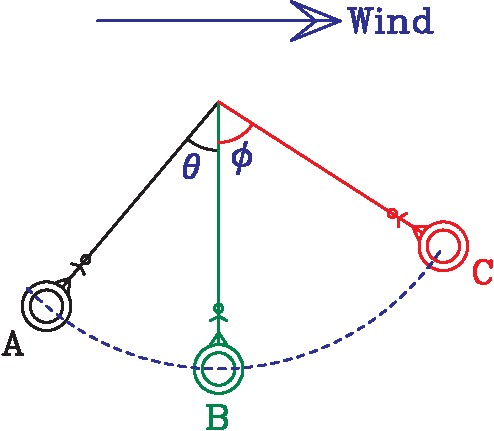
\includegraphics[width=0.9\textwidth]{swing-crop.pdf}
		\end{center}
	\end{minipage}
	
	
	

	
	
	\begin{enumerate}
		\item Find the speed of the swing at position B in terms of $F_w$, $m$, $L$, $\theta$, and $g$. In your expression for the work-energy theorem, label in words what each term represents, using language as ``kinetic energy at point A'', ``potential energy at point B'', or ``work done by wind in moving from A to B''.
		\item Write down an equation that you could solve for the angle $\phi$ in terms of $F_w$, $m$, $L$, $\theta$, and $g$. (You do not need to actually solve it.) As before, label each term that appears in your expression for the work-energy theorem.
		
		\item When the tire swings back to the left, will it stop at position $A$, will it move further to the left, or will it not reach position $A$ at all? Give an argument in words.
	\end{enumerate} 
	
	
	\vspace{0.5in}


\item A lightweight spring has a spring constant of 100 N/m and is hanging from the ceiling. Initially, the bottom of the spring is at its equilibrium position.

\begin{enumerate}
\item Someone attaches a one-kilogram mass to the spring. Its weight will make the spring stretch downward; it will bounce back and forth for a while until it comes to rest. How far below its equilibrium point will it hang?

\item While it is hanging there, someone attaches a {\it second} one-kilogram mass to the spring. It will fall down even further before the elastic force stops its fall and pulls it back upward. What is the {\it lowest point} that it will reach?

\item Again, after it oscillates for a while, it will eventually come to rest. How far below its equilibrium point will it come to rest the second time?

{\bf Hint: } {\it This problem is more subtle than it appears. Make sure you draw clear pictures of ``before'' and ``after'' scenarios when using the conservation of energy. Also, make sure you distinguish clearly from points where the mass has {\rm zero velocity} and points where it experiences {\rm zero net force}.}





	\end{enumerate}


\newpage

\item There is a section of Seneca Turnpike east of Jamesville (near Syracuse) that is about 500m long with a grade of 10\%. This means that $\tan \theta = 0.10$. As one might expect, this is difficult to ride a bike on!

\begin{enumerate} 
	\item Suppose that a cyclist and their bicycle together have a mass of 75 kg, and their legs can generate 150 watts of power for long enough to climb the hill. How fast can the cyclist ride up the hill?

	\item Suppose that the cyclist now rides back down the hill. They don't want to travel faster than 13 m/s (30 miles per hour; around 50 km/hr), so they must continually apply their brakes to reduce their speed.
	
	Brakes work by doing negative work on the bicycle; by the conservation of energy, the kinetic energy they remove from the bike is converted into heat. How many watts of heat will the cyclist's brakes generate during this process? {\it (For reference: a laptop computer generates 40 watts under very heavy load; a microwave oven may generate 2 kW.)}

\end{enumerate}
\vspace{0.5in}

\item In class, you saw a demonstration where a ball bearing (solid sphere, moment of inertia $I=\frac{2}{5}mr^2$) was rolled down a small ramp on top of a table. 


\begin{minipage}{0.5\textwidth}
	Suppose that the height of the ramp is $h$, the height of the table is $H$, and the radius of the ball is $r$.
	
	The ball rolls down the ramp, rolls across the table, and then falls off of the side of the table. Note that the ball rolls without slipping on the table (so that during this time $v = \omega r$), but this is not necessarily true once the ball leaves the table.
\end{minipage}
\hspace{0.05\textwidth}
\begin{minipage}{0.4\textwidth}
\centerline{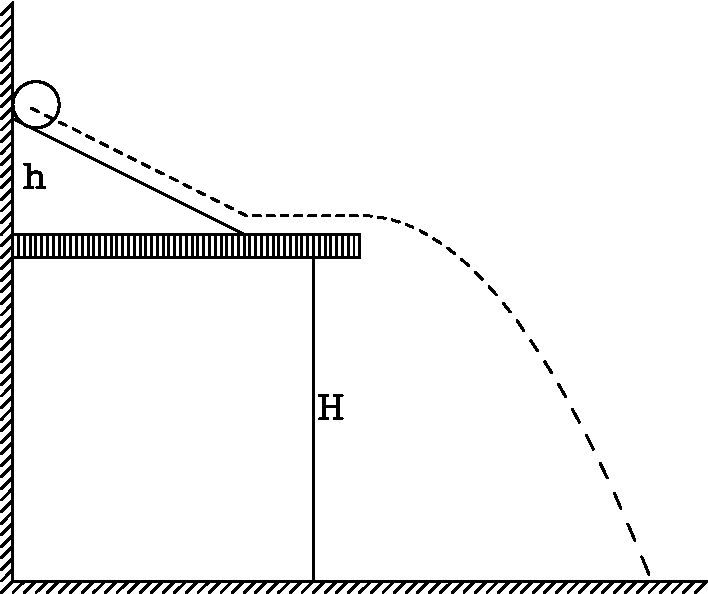
\includegraphics[width=\textwidth]{3-crop.pdf}}
\end{minipage}
\bigskip

\begin{enumerate}
	\item  How fast is the ball traveling when it reaches the edge of the table?
	\item How fast is the ball traveling when it strikes the floor? (Hint: What happens to the ball's angular velocity as it travels through the air?)
	\item How far past the edge of the table does the ball land? 
\end{enumerate}



%
%
%\begin{minipage}{0.6\textwidth}
%	A skateboarder of mass $m$ is standing on the edge of a drainage channel, as shown. The left side, where the skateboarder starts, is elevated at an angle $\theta$; the right side is elevated at an angle $\phi$. The slopes on either side are smooth, and the skateboard moves over them with essentially
%	no friction, but the flat bottom of width $b$ is covered with a little sand, and the skateboard experiences a small amount of rolling friction there, with $\mu_r$ known.
%	
%	\bigskip
%	
%	The skateboarder starts a distance $d$ up the left-hand side. They roll down the left side, across the sand-filled bottom, and up the right side.
%\end{minipage}
%\begin{minipage}{0.4\textwidth}
%	\begin{center}
%		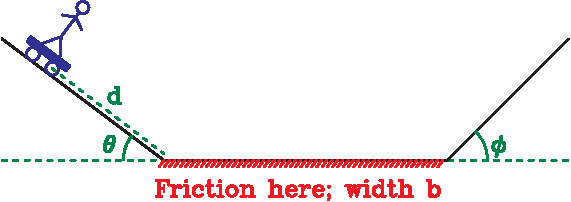
\includegraphics[width=\textwidth]{skateboarder-crop.pdf}
%	\end{center}
%\end{minipage}
%
%({\it Give your answers to the first two parts in terms of the variables above, along with $g$.})
%
%a) Determine the maximum distance $d_2$ that the skateboarder makes it up the right side. (This is the diagonal distance, not~the height.) {\it (10 points)}
%
%\vfill
%
%\begin{center} \scriptsize \it (This problem continues on the next page.)\end{center}
%\newpage
%b) After rolling up and back down the right side, the skateboarder will come back to the left side. How far will they travel back up the left side? {\it (5 points)}
%
%\vspace{3in}
%
%
%\normalsize
%\rm
%
%
%c) Suppose that you know numeric values as follows:
%
%\begin{itemize}
%	\setlength\itemsep{0.1em}
%	\item $m = 75$ kg
%	\item $\theta = 30^\circ$
%	\item $\phi = 40^\circ$
%	\item $\mu_r = 0.05$
%	\item $d = 4$ m
%	\item $b = 7$ m
%\end{itemize}
%
%How many times will the skateboarder travel across the sandy bottom of the channel before coming to rest? Explain the approach behind your solution fully. {\it (10 points)}
%
    \end{enumerate}

\end{document}
